\documentclass[dvips,12pt]{article}

% Any percent sign marks a comment to the end of the line

% Every latex document starts with a documentclass declaration like this
% The option dvips allows for graphics, 12pt is the font size, and article
%   is the style

\usepackage[pdftex]{graphicx}
\usepackage{url}
\usepackage[pdftex]{xcolor}
\usepackage{amsmath}

% These are additional packages for "pdflatex", graphics, and to include
% hyperlinks inside a document.

\setlength{\oddsidemargin}{0.25in}
\setlength{\textwidth}{6.5in}
\setlength{\topmargin}{0in}
\setlength{\textheight}{8.5in}

\newcommand{\unc}[1]
{ \delta #1 }

\newcommand{\uncsq}[1]
{ \left(\unc{#1}\right)^2 }

\newcommand{\uncratio}[1]
{ \left(\frac{\unc{#1}}{#1}\right) }

\newcommand{\uncratiosq}[1]
{ \uncratio{#1}^2 }

\newcommand{\uncvector}[1]
{ \left[ \begin{array}{c} #1 \\ \delta #1 \end{array} \right] }

\newcommand{\comment}[1]
{{\bfseries \color{red} #1}}

%----------------------------------------------------------------------------------------
%	DOCUMENT INFORMATION
%----------------------------------------------------------------------------------------

\title{2016 RPA Narrative RPA-16-10565\\
Error and Uncertainty Propagation for Fuel Cycle Calculations}

\begin{document}
\noindent\textbf{Technical Workscope Identifier:} FC-5.1b\\
\textbf{Time Frame:} 3 years\\
\textbf{Estimated Cost:} \$800,000


\section{Introduction \& Proposed Scope}
Nuclear fuel cycle simulation tools can have a large
scope of application, from the study of the
behavior of a particular type of fuel or reactor inside an
existing nuclear fleet to the prospective analysis
of a complete nuclear transition. 
Each use case
requires a specific level
of confidence, which are up to now very
poorly assessed, if assessed at all.
Indeed, the only existing way to develop confidence in
any fuel cycle calculation/tool, is to compare
with other similar tools or historical
data.  For the former, the conclusion if often 
a list of why the different software gave
different results with no conclusion on the
precision of any.  The latter only allows
validation of existing concepts and has no impact
on calculations based on the use of new
concepts.

The aim of this project is to add error
propagation capability to the CYCLUS fuel cycle
simulator \cite{CYCLUS}. Given the use case of predicting the
evolution of a large industrial enterprise in an
uncertain future, nuclear fuel cycle simulations
are generally based on approximate models and
uncertain input data.  Since strict validation is largely
considered to be impractical, such simulations are
seen as indications of trends in future behavior rather than
predictions of that behavior. Nevertheless, it
would be valuable to be able to place some
confidence bounds on those indications, both to
assess the robustness of conclusions that derive
from those indications and to provide information
about the sensitivity of those conclusions to the
uncertain data and algorithms.  Having a broad
distribution for each metric calculated in a fuel
cycle simulation instead of unique values will
allow a better comparison between different fuel
cycle scenarios.  Moreover for some critical
use cases, it could be extremely valuable to add
some degree of confidence on the results of the simulation.
This could result in confidence in the use of the tool for
such uses, and confidence in the conclusions that follow
from those results.

This project
will extend the Cyclus concept of resources to
include error information and then develop a
number of archetypes that can perform operations
to propagate that error in a manner that is 
consistent with the physical models of the 
archetype.
The ultimate calculation of fuel cycle performance
metrics will also need to be updated in order to
represent final results as distributions rather
than single values.  The primary outcome will
a demonstration of, and a
framework for, performing error propagation,
but not a comprehensive implementation of error
propagation for all models across all archetypes.
Other researchers will then be able to extend
this capability for additional archetypes, 
whether pre-existing or newly developed.

\section{Logical Path to Work Accomplishment}
The goal of this project is to add optional
extensions to Cyclus that will allow an assessment
of the error as it propagates through a fuel
cycle.  Four tasks are identified to accomplish
this goal.


\subsection{Task 1: Add uncertainty to resources}

The primary manifestation of uncertainty in a fuel
cycle simulation is in the composition of material
objects flowing through the system.  Thus the
primary task is to extend the standard Cyclus
material objects to inherently support an
uncertainty in their composition.  Each Cyclus
material is composed of both a total mass and a
vector representing the relative abundance of the
nuclides that make up that material.  While the
total mass of a material object may be subject to
some uncertainty, the composition vector is a more
interesting case.

Since these relative abundances are normalized,
the sum of a composition vector must be equal to
exactly one. Therefore, the uncertainty in the sum
must be equal to zero, the uncertainty in any one
nuclide is not independent of the uncertainty in
other nuclides.  If the mass\footnote{Cyclus 
is able to automatically and consistently switch
between mass, $\vec{m}$, and atom, $\vec{N}$, based
 definitions of a
material, and the discussion here will use 
whichever is convenient for the model being 
described.}
 of each nuclide, $i$,
is $m_i$, and its relative abundance is $f_i$,
then:

\begin{align*}
  \sum_i m_i = m_{tot} \qquad\qquad&\qquad\qquad  
       \sum_i \uncsq{m_i} = \uncsq{m_{tot}}\\
  f_i = \frac{m_i}{m_{tot}} \qquad\qquad&\qquad\qquad  
       \uncratiosq{f_i} = \uncratiosq{m_i} + \uncratiosq{m_{tot}}
\end{align*}

The data structures of a material object will be
extended to track the uncertainty in the
individual fractional abundances subject to these
relationships.

Cyclus provides a fixed set of operators for
creating and modifying material objects, largely
to ensure conservation of mass.  Most notably,
those operators include a method to divide a
material object into two and a method to combine
two material objects into one.  These operators
will each be modified to implement an algorithm
for error propagation that is appropriate to that
operator and subject to the above relationships.

When considering a material that is leaving any
given facility, there are three different sources
of uncertainty or error:
\begin{itemize}
\item the isotopic inventory vector of the input,
  $\vec{m}_{in} = m_{tot,in} \cdot \vec{f}_{in}$,
  has an associated uncertainty $\unc{\vec{m}_{in}}$,
\item the uncertainty of parameters that define that
  facility, $\tau_{p}$, 
  which correspond to the possible
  variation, or engineering tolerance, in any physics parameter, $p$,
\item the modeling error, $\epsilon_{mod}$, introduced by
  the choice of approximate archetypes models.
\end{itemize}
The uncertainty of the output material composition is a
function of all those uncertainties:
\begin{align}
  \delta \vec{m}_{out} = 
         {\cal F}\{~\unc{\vec{m}_{in}}~,~\tau_0~,~...~,~\tau_P~,~\epsilon_{mod}~\}.
\end{align}

In this work we propose to introduce archetypes
that are able to combine all those sources and
compute the resulting uncertainties on the output
materials.  The following sections indicate which
specific archetypes will be considered with some
indication of the uncertain paramters that define
those archetypes.  In some cases, these archetypes
are modifications of those that are already part
of the Cycamore set of base archetypes.  In other
cases, entirely new models will be introduced to
enable more advanced uncertainty propagation.

\subsection{Task 2: Update Cycamore archetypes for simple uncertainty propagation}

A set of standard archetypes are implemented and
distributed as part of the Cycamore package.
These archetypes use the simplest possible models
to approximate each of the facilities that they
represent.  In most cases, these models are too
simple to be the basis for a rigorous uncertainty
propagation model.  They are based heavily on user
input to approximate the physics and error
propagation may also require additional user
input.  All Cycmoare archetypes will be assessed
for their role in error propagation in a full fuel
cycle simulation, with a minimum requirement that
output material uncertainty be at least as high as
input material uncertainty.  This can be
accomplished, to a large degree, through the
correct implementation of the material object
operators referred to in the previous section.
Although further analysis will be necessary to
confirm it, this simple approach is most likely
appropriate for the source, sink
and storage facilities.

\subsubsection{Cycamore separations facility}

Some facilities require additional considerations.
The Cycamore separations facility uses a simple
separation matrix approach to distribute every
nuclide, $i$, in the input material across $K$
different streams in the output.

\begin{align}
N_{i,k} = N_{i,in} \cdot e_{i,k}
\end{align}

The only parameter which can introduce extra
variance is the separation parameter for nuclide
$i$ in output stream $k$, $e_{i,k} \pm \delta
e_{i,k}$.  For this definition of the separation
paramter, $\sum_k e_{i,k} = 1$

Assuming that the uncertainty of the input
material and the tolerance of the separation
parameters are independent, the resulting
uncertainty on the output material composition can
express as :

\begin{align}
  \uncratiosq{N_{i,k}} = \uncratiosq{N_{i,in}} +  \uncratiosq{e_{i,k}}
\end{align}

In the limit of no uncertainty in the separation
parameters, this separated materials can be
generated purely by the material operators
described in the previous section.  How to
incorporate the additional source of uncertainty,
and its impact on the uncertainty of the total
mass will be addressed in this task.

\subsubsection{Cycamore enrichment facility}

The existing Cycamore enrichment facility produces
enriched uranium on demand, matching the
enrichment of each request, $k$.  Standard models
for enrichment flow rates and separative work
requirements are used only to determine the total
throughput of the facility in any time step as a
function of the:
\begin{itemize}
\item inventory, $F_{tot}$, and composition,
  $x_f$, of feed material,
\item assay of the tails stream, $x_w$, and
\item total separative work, $S_{tot}$.
\end{itemize}

\begin{align*}
  \sum_k{F_k} \leq F_{tot}\qquad\qquad
  &\sum_k{S_k} \leq S_{tot}\\
  F_k = \frac{x_k - x_w}{x_f - x_w} P_k\qquad\qquad\qquad
  &W_k = \frac{x_k - x_f}{x_f - x_w} P_k\\
  S_k =  P_k\left(2x_k-1\right)ln\frac{x_k}{1-x_k}
         +W_k\left(2x_w-1\right)&ln\frac{x_w}{1-x_w}  
         -F_k\left(2x_f-1\right)ln\frac{x_f}{1-x_f}
\end{align*}

With this model, the uncertainty in the product
material is not determined by the inputs or the
model itself.  Instead, the uncertainty in product
enrichment can be introduced with a user-defined
tolerance parameter.  However, uncertainty in
the product enrichment can lead to uncertainty in
the amount of feed that is consumed by any request
and uncertainty in the amount of separative work
capacity that is consumed in order to fullful each
request.  A user-specified tolerance on the tails
assay can also be introduced to contribute to
these uncertainties.  The uncertainty in these 
quantities can be determined using standard
formulas for propagation of error in analytic
expressions, and are omitted here for the sake of 
brevity.

The enrichment facility contributes constraints to
the network flow problem solved by the Cyclus
dynamic resource exchange (DRE) based on the
inventory of feedstock and the available
separative work.  Since such constraints define
the feasible solution space, uncertainty in these
parameters can have an impact on the operation of
the DRE.  Further analysis will be necessary to
upgrade the DRE to accommodate such uncertainty.

The Cycamore fuel fabrication facility will
probably involve a similar level of complexity as
it combines streams of material to approximate a
desired reactivity.

\subsubsection{Cycamore reactor facility}

The reactor archetype included in Cycamore is
based on fixed matched pairs of recipes for input
and output materials that are provided by the
user, in addition of all the classical reactor
parameter (batch number, cycle length, power,
capacity factor,...).  Such a model does not allow
any meaningful way to propagate uncertainty fron
any input quantities into the output composition,
and simply requiring the user to provide uncertainty 
estimates on the output composition does not allow
any responsiveness to variations in the input
composition uncertainty.
Instead, the user will need to provide estimates
of the sensitivity of the output recipe's uncertainty to
variations in the input recipe's uncertainty.  In general, each
output isotope will be sensitive to the
uncertainty in every input isotope, although in
practice some of these can be ignored.

\begin{align}
\uncsq{N_{j,out}} = \sum_i \uncsq{N_{i,in}} \sigma_{i,j},
\end{align}
where $\sigma_{i,j}$ describes the relationship
between the uncertainty in output isotope $j$ and
uncertainty in input isotope $i$.  Since the
recipe reactor assumes a fixed input composition,
even if it does not assume a fixed uncertainty in
that composition, these sensitivity parameters can
be written to depend only on the uncertainty of
the input composition and not on the composition
itself.  

This project will include a demonstration of one
way to estimate these sensitivities using a brute
force approach.  For any given input composition,
a full depletion calculation can performed to
arrive at an output composition.  Multiple
realizations of the input composition can be
sampled from a particular uncertainty of the input
composition to yeild a population of output
compositions, from which an output uncertainty can
be measured.  If this is repeated for different
values of the input uncertainty, an approximation
of the sensitivity parameters can be performed.
The degree of approximation is consistent with
already crude approximation of the transmutation
model in the recipe reactor itself.

The Cycamore recipe reactor has many configuration
parameters that may also be uncertain.  One
example is the cycle length, typically expressed
in months.  A variation in the cycle length would
manifest itself as a variation in the burnup of
the fuel, and a similar approach to the one
described above can be used to estimate the effect
on the discharge inventory of the fuel.  A more
complete analysis of the set of parameters,
$\tau_p$, will be performed as part of this work.

\subsection{Task 3: Introduce new archetypes for advanced uncertainty propagation}

Although the basis of many fuel cycle simulators,
the recipe reactor concept is overly rigid,
unresponsive to fluctutions that may arise in fuel
compositions, particularly in the presence of
recycling.  Similarly, the simple sensitivity
approach for propagating uncertainty in the recipe
reactor is very rigid and may not respond fully to
the uncertainties that may emerge.  The next level
of sophistication relies on interpolation on a set
of precomputed results from details depletion
calculations.  In addition to a number of ongoing
efforts to introduce a variety of interpolation
approaches to Cyclus \cite{britelite, cyborg}, the
CLASS project\cite{CLASS} has developed a
stand-alone approach based on neural networks \cite{Leniau.ANE.2015}. The
CLASS methodology will be incorporated into Cyclus
modules and extended to include uncertainty
propagation.

\subsubsection{CLASS-based reactor facility}

A new reactor archetype will be introduced using
pre-trained models, ${\cal M}$, to predict key
physics parameters needed to compute the evolution
of a fuel during the irradiation. It has been
demonstrated that pre-trained neural network
models can be used to predict the evolution of the
one group cross sections of each nuclide (for
fission, capture and $n,2n$ reactions) during the
irradiation of the fuel from its initial isotopic
composition for a range of reactor concepts, from
LWR to SFR \cite{Leniau.ANE.2015, Leniau.PHYSOR.2016}.
These time-dependent cross sections are then used
by an ODE solver to determine the composition upon
discharge of the fuel.  For a neural network
predictor, ${\cal P}$, and an ODE solver, ${\cal S}$,

\begin{align}
  \vec{\Sigma}(t) &= {\cal P}\left( \vec{m}_{in}\right)\\
  \vec{m}_{out} &= {\cal S}\left( \vec{\Sigma}(t), \vec{m}_{in}\right)
\end{align}

Two approaches will be considered for extending
this neural network concept to uncertainty
propagation.

The first approach will develop a mechanism to
estimate the errors in the cross-sections, 
${\cal K}$, as a function of the initial composition:
\begin{align}
  \delta\vec{\Sigma}(t) = {\cal K}\left( \vec{m}_{in}\right)
\end{align}
and extend the ODE solver to combine the
uncertainty in the initial composition with the
error in the cross sections to estimate the
uncertainty in the final composition:
\begin{align}
  \uncvector{\vec{m}_{out}} = {\cal S^\prime}\left( \uncvector{\vec{\Sigma}(t)}, \uncvector{\vec{m}_{in}}\right)
\end{align}

Uncertainty may also be introduced in the
user-defined model parameters, $\tau_p$.  The
neural network model itself may be able to provide
insight on the uncertainty in output composition
caused by some model parameters, \textit{e.g.} he
burnup of the fuel at discharge.

The second approach will attempt to use a new
neural network predictor, ${\cal P^\prime}$, to
directly predict the fuel composition evolution:
\begin{align}
  \vec{m}_{out} = {\cal P^\prime}\left( \vec{m}_{in}\right)
\end{align}
It is also necessary to estimate the error due to
the neural network prediction:
\begin{align}
  \left(\unc{\vec{m}_{out}}\right)_{\cal P^\prime} = {\cal K}_1^{\prime}(\vec{m}_{in})
\end{align}
and the propagation of the initial uncertainty:
\begin{align}
  \left(\unc{\vec{m}_{out}}\right)_{\unc{\vec{m}_{in}}} = {\cal K}^{\prime}_2(\vec{m}_{in}, \unc{\vec{m}_{in}})
\end{align}



It's possible that this new predictor is separable
and can be decomposed into one predictor for the
final composition and another predictor for the
uncertainty in that composition.

As with the first approach, this predictor will
introduce a modeling error.

In both case, the uncertainty of the output
composition, $\vec{m}_{out}$, will have different
compoments that need to be computed and combined:
\begin{align}
  \uncratiosq{\vec{m}_{out}}_{tot} =
  {\cal C}\left(  \uncratiosq{\vec{m}_{out}} _{\cal M},
                  \uncratiosq{\vec{m}_{out}} _{\delta \vec{m}_{in}},
                  \uncratiosq{\vec{m}_{out}} _{\vec{\tau}}
         \right)
\end{align}

In both case, we are proposing to determine and
combine those errors using empirical methods.

\paragraph{The Modeling Error $\uncratiosq{\vec{m}_{out}} _{\cal M}$ : \\}

Since both cases rely on neural networks that are
trained with sets of training data, modeling
errors arise from errors in the methods of
producing those training data and also in the
methods of training the neural network.  For this
work, errors in the underlying training data will
be ignored, but errors in the neural network
algorithms can be empircally estimated by
comparing the predictions of the neural network to
a direct calculation for data sets that are not in
the set of training data.

For the first approach, the neural network will be
predicting cross sections at each time step of a
depletion solve based on the initial composition,
and each such prediction has an associated
modeling error.  Different ODE solver approaches
will be investigated for their ability to include
the combination of uncertainty and modeling error
as the solution progresses through time.  There is
also a second order effect that the magnitude of
the modeling error in the cross-sections may
depend on the magnitude of the uncertainty in the
initial material composition.  Such effects will
be investigated but may not be included in the
final methodology.

In the second approach, we will aim to directly
predict the final composition and its uncertainty
from the initial composition and its uncertainty
using the neural network.


This error are more complicated in the first case
than in the second case. Indeed in the second case,
the Modeling Error are the direct error on the
prediction made by the neural networks.


In the first case, those prediction errors have to
be propagated along the depletion calculation.
In both cases, after having trained the neural
network, we need to map the error on the neural
prediction.
To do so, to detect neural network over-training,
the best is to compute a new data set, similar but
independant to the one use for the training, and
test the accuracy of the neural network prediction.
Then using an interpolation model (as kriging or
neural network), ${\cal K}_k$,  predict the error
on the parameter predictions, $\rho_k$, made with
the neural network :
\begin{align}
  \left( \frac{\delta \rho_k}{\rho_k} \right)^{2} _{{\cal M}} = {\cal K}_k \left( \vec{m}^{i} \right)
\end{align}

For the second the case the estimation of the
direct Modeling Error end there, as $\rho_k$ = $m_k$.

For the first case, the predicted paramter are the
one group cross section, one still need to
propagate those error during the depletion
calculation ${\cal D}$.\\
The Bateman equation can be written in its matrix
form as :
\begin{align}
  \frac{d\vec{N}}{dt}(t) = (\Lambda + \phi(t) . D) \times \vec{N}(t)
\end{align}
where $\vec{N}(t)$ represents the isotopic vector
of the fuel at the time t and
$\frac{d\vec{N}}{dt}(t)$ its variation, $\Lambda$
the decay part of the depletion matrix, $D$ the
cross section part and $\phi(t)$ the neutron flux.
The neutron flux can be estimated assuming a the
constant power in the reactor core as:
\begin{align}
  \phi(t) = \frac{P}{ \vec{E}_f \times D_f \times \vec{N}(t)},
\end{align}
with P the thermal power of the core, $\vec{E}_f$,
the vector of the energy release per fission and
$D_f$ the fission compoment of the cross section
matrix.

The depletion calculation will be performed with a
step by step process, considering the one group
cross section are constant during a step. As this
kind of error is commun to any step by step
depletion calculation and inversely correlated
with he timestep length, in first approximation
its effect will not be included in our calculation
and could be reduce with a proper choice of the
timestep length. \\
As a finit number of one group cross section will
be predicted, a brief study will be conducted to
estimate the impact of ignoring some reactions and
a reaction rate threshold will be set to have a
negligible impact on the resulting depletion
calculation error.\\

As the cross section matrix at any time t, $D(t)$,
can be determine using the prediction of the
neural network (from the initial fuel composition)
, it possible to determinate the sensitivity,
$\gamma_{i,j}$  of the one group cross section,
$i$ on the isotope quantity, $j$ at the end of the
depletion step, $k$. One can then express the
modeling error at the end of the step $k$ as :
\begin{align}
  \left( \frac{\delta m_j^{k}}{m_j^{k}} \right)^{2} _{{\cal M}} = \sum_{i}\left( \frac{\delta \sigma_i^{k-1}}{\sigma_i^{k-1}} \right)^{2} *\gamma_{i,j}(k)\label{eq:mod}
\end{align}
Following the same reasonment one can establish
also the sentivity $\beta_{ij}$ of the initial
uncertainty on the isotope, $j$ on the isotope,
$i$, uncertainty at the end of the time step $k$
as:
\begin{align}
  \left( \frac{\delta m_i^{k}}{m_i^{k}} \right)^{2} _{\delta \vec{m_i}^{k-1} } = \sum_{u}\left( \frac{\delta m_u^{k-1}}{m_u^{k-1}} \right)^{2} *\beta_{u,j}(k) \label{eq:dm}
\end{align}



Combining together the equation \eqref{eq:mod} and
\eqref{eq:dm} will allow us to propagate the
modeling uncertainty through the integration of
the Bateman equation. Because we are able to
predict the cross section and the associated
prediction error from the initial composition, so
the effect of the error on the cross section at
the time step $k$ is already included in the error
on the one group cross section of the time step
$k+1$.

%and then on the final composition (considering $L$ calculation step) as :
%\begin{eqnarray}
%  \nonumber
%  \left( \frac{\delta \vec{m}^{L}}{\vec{m}^{L}} \right)^{2} _{Mod} &=& \sum_{i} \left( \frac{\delta \sigma_i^{L-1}}{\sigma_i^{L-1}} \right)^{2} *\gamma_{i,j}(L)\\
%\nonumber
%  &+& \sum_{u^{0}}  \sum_{i} \left( \frac{\delta \sigma_i^{L-2}}{\sigma_i^{k-2}} \right)^{2} *\gamma_{i,u^{0}}(L-1) *\beta_{u^{0},j}(L)\\
%\nonumber
%&+& \sum_{u^{0}} \sum_{u^{1}} \sum_{i} \left( \frac{\delta \sigma_i^{L-3}}{\sigma_i^{L-3}} \right)^{2} *\gamma_{i,u^{1}}(L-2) *\beta_{u^{1},u^{0}}(L-1) *\beta_{u^{0},j}(L)\\
%\nonumber
%&+& ...\\
%  &+& \sum_{u^{0}}... \sum_{u^{L-2}} \sum_{i} \left( \frac{\delta \sigma_i^{0}}{\sigma_i^{0}} \right)^{2} *\gamma_{i,u^{L-2}}(1)*\beta_{u^{L-2},u^{L-3}}(2)* ...  *\beta_{u^{0},j}(L)
%\end{eqnarray}



\paragraph{The Initial Composition Uncertainty propagation:\\}
Based on the previous formalisum definited, one
can consider the initial composition uncertainty
as term $\left( \frac{\delta m_i^{0}}{m_i^{0}} \right)^{2}$
and then be easely included in the error
propagation  at the first step as :\\
\begin{align}
  \left( \frac{\delta m_i^{1}}{m_i^{1}} \right)^{2} = \sum_{u}\left( \frac{\delta m_u^{0}}{m_u^{0}} \right)^{2} *\beta_{u,j}(1) + \sum_{i}\left( \frac{\delta \sigma_i^{0}}{\sigma_i^{0}} \right)^{2} *\gamma_{i,j}(1) \label{eq:dm0}
\end{align}



One also need to convolute the uncertainty on the
initial composition with the model prediction.
One can need to extend the ${\cal K}$ interpolation method to isotopic composition uncertainty :
\begin{align}
  \left( \frac{\delta \rho_k}{\rho_k} \right)^{2} _{{\cal M}, \delta \vec{m}^{i}} = {\cal K}_k \left( \vec{m}^{i} , \delta\vec{m}^{i} \right)
\end{align}
This could be easly be done statistically:
determining the distribution of the outut
parameter and its error running many time the
predictiv model, ${\cal M}$, and the error
interpolator, ${\cal K}$, on a wild varity of
isotopic composition ranged inside the initial
composition uncertainty.

\paragraph{Other error:\\}
We are aware that the error listed previously are
not exhaustiv. For exemple, the neural network
will be trained on simulated data which are
subject to many different error/uncertainty
(nuclear data uncertainty, statistical error,
modeling error...). We will consider those errors
beyond the scope of this study.
The aim of this project is to create a framework
for uncertainty/error propagation in fuel cycle
calculation and develop the require tool to do so.
Therefore one will only consider the error induce
by the developed tools.


%Again using an statistical approach, one will be
%able to assess the impact of the isotopic
%composition uncertainty on the one group cross
%section prediction error: running many time the
%neural network prediction and the ${cal K}$ error
%interpolator, one could determine the resulting
%one group cross section and the



%Because the predictive model will be able to
%predict the one group cross section as the
%function of time (or burnup), one should be able
%to propagate those error using sensitivity
%analysis.  \comment{PPHW: we need more here - this
%  is the key contribution.}

%The time discretization other other approximations
%required to solve the Bateman equation will
%introduce computation error that also needs to be
%incorporated into the final uncertainty. This
%contribution to uncertainty can be characterized
%by a comparison of depletion calculations
%performed with this approach with a reference
%depletion calculation using the same modeling
%approach used in the training depletions, along
%the full isotopic space.


%It may also be possible, and preferable, to train
%the neural network to directly predict the final
%isotopic inventory from the initial isotopic
%inventory and other reactor parameters.  Although
%this approach has not been demonstrated, even in
%the absence of uncertainty, it may provide a
%better platform for the propagation of
%uncertainty.

%\comment{PPHW: I am not really sure what this
%  looks like, and the following text spends a lot
%  of time discussing what we WON'T do.}

%The main reason leading the try of direct
%prediction of the isotopic evolution, is the
%error/uncertainty propagation. As express
%prevsiously :

%\begin{align}
%\delta \vec{m}_{out} = {\cal F}\{~\delta\vec{m}_{in}~,~\tau_0~,~...~,~\tau_P~,~\epsilon_{mod}~\}
%\end{align}
%The determination and the propagation of all
%uncertainty source is, for this kind of reactor, a
%complicated matter. The error due to the
%computation of the depletion calculation are wild:
%\begin{itemize}
%\item the error of the neural network predictor,
%  $\epsilon^{nn}_{i}$, with $i\in[0..N]$, $N$ the
%  number of predicted parameter,
%\item the convolution of the uncertainty on the
%  material composition with the neural network
%  prediction.
%\item the calculation error on the data sets used
%  to train the neural network, $\epsilon_{T.D.}$.
%\end{itemize}
%And then can be expressed as :
%\begin{align}
%\epsilon_{mod} = {\cal G}\{~\delta\vec{N}_{in}~,~\epsilon^{nn}_{0}~,~...~,~\epsilon^{nn}_{n}~,~\epsilon_{T.D.}~\}
%\end{align}

%Because, the predictive model are trained on
%sample populated using few thousand of depletion
%calculation, which are subject to computation
%error, $\epsilon_{T.D.}$. On one side, a depletion
%calculation take as input, the nuclear data. Those
%nuclear data are interpolated/extrapolated from
%many different experimental measurement using many
%different models. Therefore the nuclear data
%contain uncertainty...  Those uncertainty are
%extremely difficult to propagate properly through
%a full depletion calculation because of the
%coupling between neutron transport and depletion
%calculation: the composition of the fuel impact
%the shape of the neutron spectrum, which impact
%the reaction rate on the nuclei... On the other
%side, the depletion calculation require different
%approximation to be completed. There is nearly
%impossible using Monte Carlo technique on a PWR
%full core calculation due to source convergence
%issue. It is also extremely complicate to follow
%precisely the different reactor parameter, such as
%boron concentration, rod control management,
%charge factor evolution, neutron leakage... The
%study and the propagation of the modeling
%uncertainty, such as the modeling simplification
%and the nuclear data uncertainty is way beyond the
%scope of this project...\\
%This require a full dedicated research project
%(and probably more). Therefore, those error,
%$\epsilon_{T.D.}$, will not be considered on the
%first version of this work. This might need to be
%reconsidered when the depletion calculation error
%propagation capacity will have done important
%progress.\\
%The direct error induced by the use of predictive
%model, $\epsilon^{nn}_{i}$ on each parameter, $i$,
%need to be assessed. This could be performed with
%a mapping the error on the isotopic space
%populated with the training sample. This will
%allow to determine the error of the model on each
%point on the isotopic space populated. We might
%use then a other neural network, or other
%interpolation method to predict the error of the
%prediction as the function of the isotopic
%composition.\\
%Once we have a working predictive model and a map
%of the error on the prediction, one need to build
%the covariance matrix which will allow to
%convolute the uncertainty on the input material,
%$\delta N_{in}$, with the prediction of the
%model.\\


\subsubsection{CLASS-based fuel fabrication} \label{sec:fabrication}

The aim of the fuel fabrication is to mix
different incoming material streams in order to
build a fuel composition that supports the
neutronics/physics requirement of the reactor. The
Cycamore fuel fabrication facility mixes two
streams of material using an equivalence method to
approximate a desired composition by matching its
initial reactivity.  \cite{cycamore_fab}
\comment{PPHW: may need to tweak this wording
  about Cycamore to be concise and correct.}  By
contrast, methods implemented in the CLASS project
have used a similar neural network approach as
described above to determine how to mix multiple
streams of material in order to satisfy a number
of reactor performance goals including initial
reactivity, burnup and/or conversion ratio.


What existe now :
\begin{align}
  \rho = {\cal P^{\star}}\left( \vec{m}_{1},\vec{m}_{2}, BU \right)
\end{align}

It is also necessary to estimate the error due to
the neural network prediction:
\begin{align}
  \left(\unc{\rho}\right)_{\cal P^\star} = {\cal K}_1^{\star}\left( \vec{m}_{1},\vec{m}_{2}, BU \right)
\end{align}
and the propagation of the initial uncertainty:
\begin{align}
  \left(\unc{\rho}\right)_{\unc{\vec{m}_{1}},\unc{\vec{m}_{2}}} = {\cal K}^{\star}_2\left( \uncvector{\vec{m}_{1}},\uncvector{\vec{m}_{2}}, BU \right)
\end{align}
We may consider directly include $\delta BU$:
\begin{align}
  \left(\unc{\rho}\right)_{\unc{\vec{m}_{1}},\unc{\vec{m}_{2}},\unc{BU}} = {\cal K}^{\star}_2\left( \uncvector{\vec{m}_{1}},\uncvector{\vec{m}_{2}}, \uncvector{BU} \right)
\end{align}

We are considering in the first time including
fabrication model for MOX fuel only, in LWR and
SFR, used as burner and breeder for SFR. One will
use algorithm building fuel allowing to build fuel
reaching the targeted burnup according to either
criticality criterium either conversion ratio
criterium.  Those algorithm will relies on the
capabilities of some predictive model to predict
the maximal achievable burnup depending on the the
criticality or conversion ratio evolution
according to burnup.  The predictive model as the
reactor model, will be based on the use of neural
network formerly trained on the same set of
training depletion calculation used for the
reactor models. The capability of the neural
network have been proven to predict the evolution
of the criticality in PWR reactor using MOX fuel
\cite{Leniaux.NN, CLASS_UserManual}, as well as
the the initial criticality of MOX fuel in SFR
\cite{CLASS UserManual} and should be possible to
extend it to conversion ratio evolution.

The error/uncertainty propagation for fuel
fabrication should be pretty similar than for
reactor. Indeed the uncertainty can be expressed
as :
\begin{align}
\delta \vec{N}_{out} = {\cal H}\{~\delta\vec{N}_{in}~,~\epsilon_{mod}~\}.
\end{align}
In this case there is no tolerance, since the
parameter are goal to achieve, not physicals
characteristics. As well as previously the error
of the model can be expressed as :
\begin{align}
\epsilon_{mod} = {\cal K}\{~\delta\vec{N}_{in}~,~\epsilon^{nn}_{0}~,~...~,~\epsilon^{nn}_{n}~,~\epsilon_{T.D.}~\},
\end{align}
 where $\epsilon^{nn}_{i}$ represent the error on
 the prediction of the parameter $i$ by the neural
 network predictive model and $\epsilon_{T.D.}$
 the error due to the error on the depletion
 calculation composing the training set, which
 will not be considered since we dont have any way
 to correctly estimate it.\\
 
 As for the reactor model, the $\epsilon^{nn}_{i}$
 component of the error can be determined through
 a mapping of the error along the isotopic space,
 and the impact of the material input uncertainty
 needed the be assessed by the calculation of the
 covariance matrix which need to be build.

\subsection{Task 4: Demonstrate uncertainty propagation}
During the realization of this work we would like
to validate each step of the uncertainty
propagation process. First, with a mid/early-term
validation, after the enrichment facilities, the
separation and the recipes reactor will be
implemented, it will be possible to confirm the
uncertainty is correctly propagated, using a brute
force validation (with the "Total Monte Carlo"
method). This validation will be continued with
new archetypes will be implemented in CYCLUS...\\
An other gaol we want to achieve, is an
sensitivity analysis, allowing to determine the
impact of the different
uncertainty/error/tolerance on the final
calculation uncertainty. This should allow to
define precisely where the future effort should be
focus to reduce those uncertainty sources
accordingly to the object of the calculation and
also to validate (or un-validate) the use of fuel
cycle simulation tool for some specialized study
(such as non-proliferation study...)\\
With all the necessary components in place, a
series of demonstration simulations will be
conducted using fuel cycles of increasing
complexity: once through, MOX LWR recycle, and
fast reactor recycle.  These scenarios will be
constructed to highlight the role of error and
uncertainty and identify metrics in which the
presence uncertainty may impact fuel cycle
analysis conclusions.



%\textit{We imagine 3 step in the final
%phase. First we would like to step up a testing
%mechanism, based on simply brute force the
%uncertainty propagation in the fuel cycle
%calculation by using some kind of Total monte
%Carlo, allowing all parameters to fluctuate
%accordingly to their respective uncertainty on
%many integration of the same calculation. The
%result distribution can be read as a direct
%measure of the uncertainty on the final parameter
%and will be compared to the direct uncertainty
%propagation calculation as a validation of all
%the method previously presented. This method will
%(turning on the uncertainty on each parameter one
%by one) to validate the uncertainty propagation
%on each parameter...\\

%One need nevertheless keep in mind that
%everything is never perfect, and one should
%always try to improve. To do so it is required to
%identify the most problematic issue and solve
%it. In this particular case, one need to identify
%what is the uncertainty gaol depending on the
%application of the fuel calculation, of course
%the precision goal is very different when one
%doing a prospective calculation versus a
%non-proliferation retrospective
%analysis... Knowing it, one very important of
%this project is it could allow through
%sensitivity analysis to identify the biggest
%uncertainty source, and help to focus to improve
%it.\\ 

%That is why, in addition of the TMC test tool, I
%would like to develop a tool/method to
%systematically allows user to perform sensitivity
%analysis applied to their calculation allowing us
%to improve future models dedicated to some
%precise use of the CYCLUS tool.\\

%Finally, we would like
%Third step : application to simple case : PWR, transition from PWR to FBR...}
\section{Relevance of Proposed Research}
This proposal aims to provide an important feature
needed in the fuel cycle simulator.  Given the
appropriate estimation of the error relative to
any fuel cycle simulation, the simulator would be
able to make decisions about fuel cycle transition
like fuel reprocessing, or the launching of new
technologies or types of reactors. Furthermore,
the project will be one of the first of its kind
to introducing error propagation in fuel cycle
calculation, increasing the utility of the Cyclus
kernel. Since the precision of fuel cycle tool
have never been assessed, this work might the
first step providing more confidence in the fuel
cycle calculation. And even if this wok will be
applied to the fuel cycle simulation tool CYCLUS,
the concept should be a theoretically applicable
on any agent based fuel cycle simulation
tool.\\ 
Additionally, new archetypes will be contributed
to the Cyclus ecosystem, including not only error
propagation but also different fuel fabrication
methods, cross-section prediction models and a
Bateman equation solver. These features will
permit future comparison between the different
fuel fabrication models and improve the user
experience and confidence in the interpretations
of Cyclus simulations.

\pagebreak
\section{Milestone Task Listing}
This research project consist in four major tasks
that could be conducted in parallel.  The first
one will be very short ($<$ 6 month), dedicated to
update CYCLUS and allow it to handle
uncertainty. The second one should be the longer
task (12 - 24 months) where the models will be
developed. The predictive model development
can/should/will be started at the start of the
project. The third will be started after the end
of the TASK 1 and corresponds to CYCLUS archetypes
update and included in a separated package. The
development of some archetypes will depends on the
progress on the TASK2. The last task is the
validation and application one and will be started
with the completion of the different
TASK3-subtasks. The ideal progression is
represented on the figure \ref{fig:progression}.
\begin{figure}[h!]
\centering
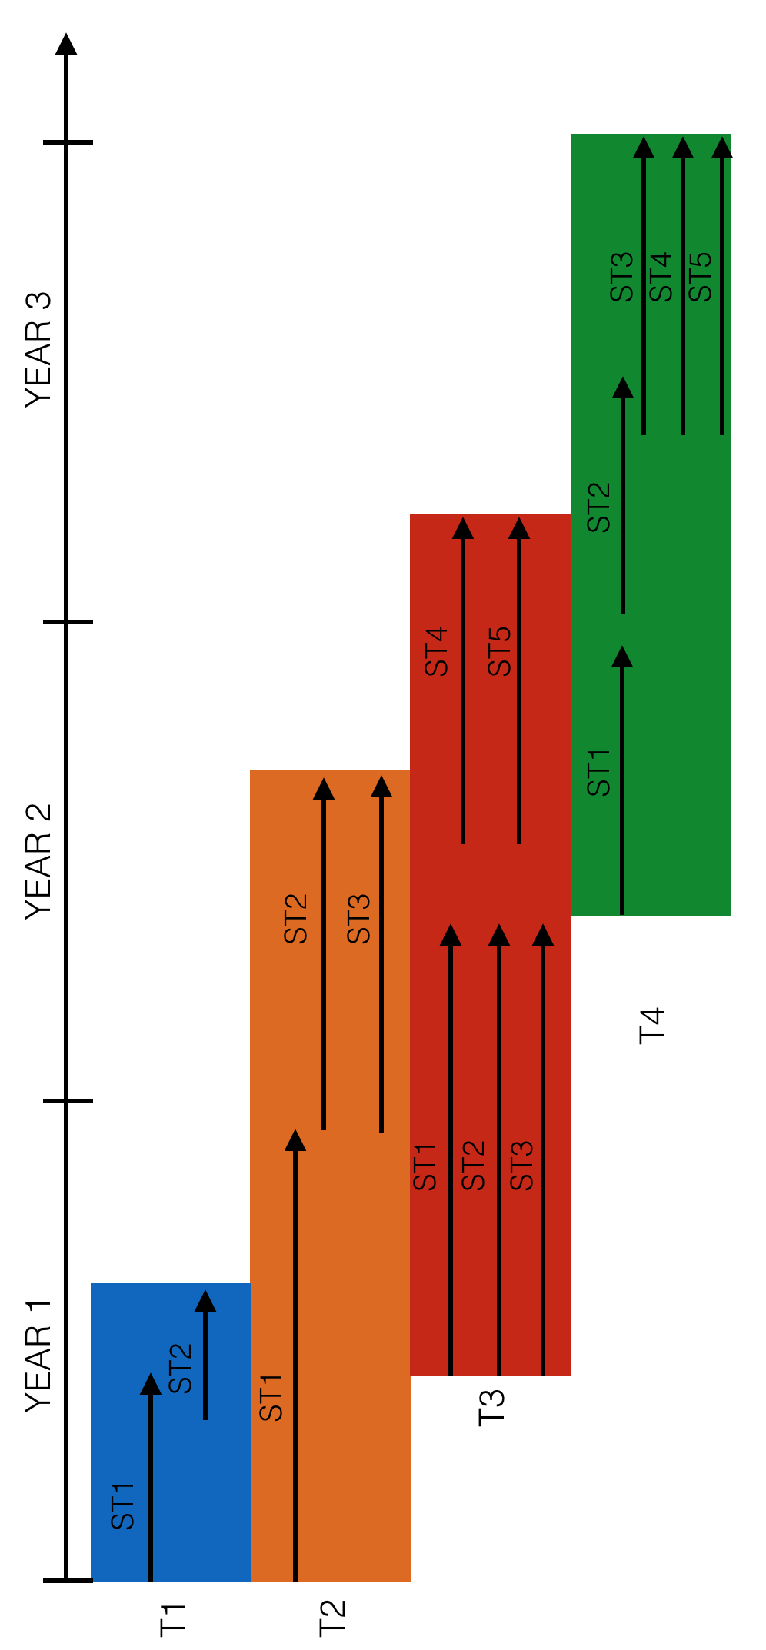
\includegraphics[angle=270,width=1\textwidth]	{TIMESCHEDULE}
\caption{Preliminary schedule of the project, with the different Task (T\#) (1 in blue, 2 orange, 3 red, 4 green) and the corresponding subtask (SB\#).}
\label{fig:progression}
\end{figure}

\noindent\textbf{TASK 1:} CYCLUS update for uncertainty awareness
\begin{itemize}
\item subtask 1: update material to uncertainty,
\item subtask 2: validate the backward
  compatibility,
\item subtask 3: Add a default uncertainty
  behavior when using both uncertainty aware
  archetypes and standard one in the same time ?
\end{itemize}

\noindent\textbf{TASK 2:} Updating the CYCLUS Archetypes to uncertainty management
\begin{itemize}
\item subtask 1: enrichment facility, 
\item subtask 2: separation facility,
\item subtask 3: recipe reactor,
\item subtask 4: reactor archetypes, depletion
  calculation/prediction, uncertainty propagation,
\item subtask 5: fuel fab archetypes, mixing
  calculation/prediction, uncertainty propagation.
\end{itemize}

\noindent\textbf{TASK 3:} Modeling development
\begin{itemize}
\item subtask 1: isotopic space definition,
  training sample realization
\item subtask 2: reactor models development:
  parameter prediction, error analysis
\item subtask 3: fuel fabrication model
  development: parameter prediction, error
  analysis
\end{itemize}
 
\noindent\textbf{TASK 4:} Validation \& application
\begin{itemize}
\item subtask 1: validation of the overall process
  with simple calculation : enrichment +
  separation + recipe reactor
\item subtask 2: validation of modeling
  capabilities (Fab + reactor)

\item subtask 3: exemple calculation: PWR,
  transition from PWR to FBR
\item subtask 4: full sensitivity analysis

\item subtask 5: time dependent parameters
  sensitivity analysis (discharge burnup, capacity
  factor...)

\item subtask X: comparison with other physic
  modeling capabilities such as Bright-Lite ?
\end{itemize}






 







%----------------------------------------------------------------------------------------
%	BIBLIOGRAPHY
%----------------------------------------------------------------------------------------

\bibliographystyle{unsrt}

\bibliography{Uncertainty}

%----------------------------------------------------------------------------------------


\end{document}
